\documentclass[12pt, a4paper]{article}

\usepackage[utf8]{inputenc}
\usepackage{mathtools}
\usepackage{amssymb}
\usepackage{ntheorem}
\usepackage[framemethod=TikZ]{mdframed}
\usepackage{amsmath}
\usepackage[hidelinks]{hyperref}
\usepackage{cleveref}
\usepackage[most]{tcolorbox}
\usepackage{fancyhdr}
\usepackage{lastpage}
\usepackage{geometry}
\usepackage{graphicx}
\usepackage{float} 
\usepackage{subfigure} 
\usepackage{arydshln}
\usepackage{multicol}
\usepackage{url}
\usepackage{setspace}
\usepackage[T1]{fontenc}
\usepackage{mathptmx}
\usepackage{framed}
\usepackage{xcolor}
\usepackage{chemfig}

\geometry{a4paper, left=2cm, right=2cm, bottom=2cm, top=2cm}

\definecolor{blue}{RGB}{0, 47, 167}
\definecolor{red}{RGB}{238,34,12}
\definecolor{green}{rgb}{0,0.42,0.24}
\definecolor{orange}{RGB}{242,169,0}

\theorembodyfont{\rmfamily}
\newtheorem{und}{U}[subsection]
\newtheorem{skl}{S}[subsection]
\newtheorem{app}{A}[subsection]
\newtheorem{que}{Q}[subsection]
%\newtheorem{lemma}{Lemma}[subsection]
%\newtheorem{prop}{Proposition}[subsection]
%\newtheorem{conj}{Conjecture}[subsection]
%\newtheorem{remark}{Remark}[subsection]
%\newtheorem{proof}{Proof}[subsection]

\rhead{\thepage}
\linespread{1.15}

\title{\textbf{Biology HL}}
\author{Jiuru Lyu}
\date{\today}

%\def\Z{{\mathbb{Z}}}
%\def\R{{\mathbb{R}}}
%\def\C{{\mathbb{C}}}
%\def\Q{{\mathbb{Q}}}
%\def\E{{\mathbb{E}}}
%\def\d{{\mathrm{d}}}
%\def\i{{\mathrm{i}}}
%\def\RE{{\mathrm{Re}}}
%\def\IM{{\mathrm{Im}}}
%\def\Arg{{\mathrm{Arg}}}
%\def\cis{\mathrm{cis}}

\begin{document}

\maketitle
\tableofcontents

\newpage

\section{Cell biology}
\subsection{Introduction to cells}
\begin{und}
    According to the cell theory, living organisms are composed of cells.
\end{und}
\begin{und}
    Organisms consisting of only one cell carry out all functions of life in that cell.
\end{und}
\begin{tcolorbox}\begin{que}
    \textbf{Describe the \color{red}{cell theory}.}
        \begin{enumerate}
            \item All living things are made of cells.
            \item Cells are the smallest unit of life.
            \item Cells come from pre-existing cells.
        \end{enumerate}
\end{que}\end{tcolorbox}
\begin{app}
    Questioning the cell theory using atypical examples, including striated muscle, giant algae and aseptate fungal hyphae.
\end{app}
\begin{enumerate}
    \item Muscle cells
    \begin{itemize}
        \item Have more than one nucleus per cell. - {\color{blue}{challenges the idea that a cell has one nucleus.}}
        \item They are surrounded by a single plasma membrane, but they are multi-nucleated. 
        \item Contain fibers that can be very long. 
    \end{itemize}
    \item Fungal cells
    \begin{itemize}
        \item Develop without division of the cytoplasm - {\color{blue}{challenges the idea that a cell is a single unit}}
        \item Fungal hyphae: very large with many nuclei and a continuous cytoplasm. 
    \end{itemize}
    \begin{figure}[H]
        \center
        \includegraphics[width=0.5\textwidth]{fig1.1.png}
    \end{figure}
\end{enumerate}
\begin{skl}
    Use of a light microscope to investigate the structure of cells and tissues, with drawing of cells. Calculation of the magnification of drawings and the actual size of structures and ultrastructures shown in drawings or micrographs. (Practical 1)
    $${\color{red}{\text{Magnificantion}=\frac{\text{Size of image}}{\text{Size of actual specimen}}}}.$$
\end{skl}
\begin{app}
    Investigation of functions of life in \textit{Paramecium} and one named photosynthetic unicellular organism.
\end{app}
\begin{enumerate}
    \item Microorganism/Unicellular organisms: 
    \begin{itemize}
        \item Archae
        \item Bacteria
        \item Paramecium
        \item Yeast
    \end{itemize}
    \item Functions of life: 
    \begin{itemize}
        \item Metabolism
        \item Response
        \item Homeostasis
        \item Growth
        \item Reproduction
        \item Nutrition
        \item Excretion
    \end{itemize}
\end{enumerate}
\begin{tcolorbox}\begin{que}
    \textbf{Compare the function of life of \textit{Paramecium} and \textit{Chlamydomonas}.}
    \begin{enumerate}
        \item \textbf{\color{red}{Metabolism}}: Both contain many enzymes to catalyze many reactions. 
        \item \textbf{\color{red}{Homeostasis}}: Both regulate their internal volume of water. 
        \item \textbf{\color{red}{Nutrition}}: \textit{Paramecium} feeds by smaller organisms by ingesting, and \textit{Chlamydomonas} does photosynthesis. 
        \item \textbf{\color{red}{Excretion}}: \textit{Paramecium} excretes CO$_2$, and \textit{Chlamydomonas} excretes O$_2$ by photosynthesis. 
    \end{enumerate}
    \textbf{Exam Tips: }
    \begin{itemize}
        \item \textbf{\color{orange}{Comparison}} needs to contain both similarities and differences of the two objects. 
        \item \textbf{\color{orange}{Distinguish}} only needs to contain differences of the two objects, correspondingly. 
    \end{itemize}
\end{que}\end{tcolorbox}
\begin{und}
    Surface area to volume ratio is important in the limitation of cell size.
\end{und}
\begin{tcolorbox}\begin{que}
    \textbf{Why are cells in microscopic level? }
    \begin{enumerate}
        \item The ratio of heat production/waste production/resource consumption of a cell is a function of volume. 
        \item The rate of exchange materials, and energy (heat) is a function of the cell's surface area. 
    \end{enumerate}
\end{que}\end{tcolorbox}
\textbf{Multicellular and Differentiation: }
\begin{enumerate}
    \item \begin{und} Multicellular organisms have the properties that emerge from the interaction of their cellular components. \end{und}
    \item Emergent properties arise from the interaction of components parts: {\color{red}{The whole is greater than the sum of its parts}}.
    \item \textbf{\color{red}{Differentiation}}: a cell having a specific function. 
    \item \begin{und} Specialized tissues can develop by cell differentiation in multicellular organism \end{und}
    \item \begin{und} Differentiation involves the expression of some genes but not others in a cell's genome. \end{und}
\end{enumerate}
\textbf{Stem Cells: }
\begin{enumerate}
    \item \begin{und} The capacity of stem cells to divide and differentiate along different pathways is necessary in embryonic development and also makes stem cells suitable for therapeutic uses.\end{und}
    \item \textbf{\color{red}{Stem cells}} retain the ability to divide, and they are undifferentiated cells that have not activated their genes. 
    \item \begin{app} Use of stem cells to treat Stargardt's disease and one other named condition. \end{app}
    \begin{itemize}
        \item \textbf{\color{red}{Stargardt's disease}} is a type of genetic disease. 
        \item Another named condition could be \textbf{\color{red}{Leukemia}}, a type of cancer. 
    \end{itemize}
    \item \begin{app} Ethics of the therapeutic use of stem cells from specially created embryos, from the umbilical cord blood of a newborn baby and from an adult's own tissues. \end{app}
\end{enumerate}

\subsection{Ultrastructure of cells}
\begin{und}
    Electron microscopes have a much higher resolution than light microscopes. 
\end{und}
\begin{enumerate}
    \item Def: \textbf{\color{red}{Resolution}} is the measure of the clarity of the image, or the minimum distance of two distinguishable points. 
    \item The smaller the resolution, the better the microscope. 
\end{enumerate}
\begin{und}
    Prokaryotes have a simple cell structure without compartmentalization. 
\end{und}
\begin{skl} Drawing of the ultrastructure of prokaryotic cells based on electron micrographs. \end{skl}
\begin{multicols}{2}
\begin{figure}[H]
        \center
        \includegraphics[width=0.45\textwidth]{fig1.2.png}
\end{figure}
Functions: 
    \begin{itemize}
        \item \textbf{\color{red}{Cell wall}}: protection
        \item \textbf{\color{red}{Plasma membrane}}: controlling the entry and exist of substances, pumping some of them by active transport. 
        \item \textbf{\color{red}{Cytoplasm}}: site of metabolic reactions
        \item \textbf{\color{red}{Ribosomes}}: synthesis of proteins
        \item \textbf{\color{red}{Nucleoid/Nuclear region}}: DNA controls the cell's function
        \item \textbf{\color{red}{Flagellum}}: movement
        \item \textbf{\color{red}{Pili}}: attachment to other surface and other bacteria during reproduction
        \item \textbf{\color{red}{Plasmids}}: extra chromosomal material
    \end{itemize} 
\end{multicols} 
\begin{und}
    Eukaryotes have a compartmentalized cell structure. 
\end{und}
\begin{skl}
    Drawing of the ultrastructure of eukaryotic cells based on electron micrographs.
\end{skl}
\begin{figure}[H]
    \center
    \includegraphics[width=0.5\textwidth]{fig1.3.png}
\end{figure}
\begin{app}
    Structure and function of organelles within exocrine gland cells of the pancreas and within palisade mesophyll cells of the leaf.
\end{app} 
\begin{itemize}
    \item \textbf{\color{red}{Rough endoplasmic reticulum (rER)}}: synthesis of proteins to be exported outside of the cell. 
    \item \textbf{\color{red}{Ribosomes}}: synthesis of proteins for the rER system or for cell own's function
    \item \textbf{\color{red}{Golgi apparatus}}: manufacturing/transforming/maturing proteins from the ER. 
    \item \textbf{\color{red}{Vesicles}}: transport different materials within the cell
    \item \textbf{\color{red}{Lysosome}}: contain digestive enzymes, do cell digestion
    \item \textbf{\color{red}{Mitochondria}}: produces ATP
    \item \textbf{\color{red}{Nuclear pore}}: allow materials to go in and out the cell
    \item \textbf{\color{red}{DNA}}: control the cell function
    \item \textbf{\color{red}{Nuclear envelope}}: maintain the DNA separated from the rest of the cell - {\color{blue}{DNA cannot survive in the cytoplasm.}}
    \item \textbf{\color{red}{Cytoplasm}}: place of metabolic reactions
    \item \textbf{\color{red}{Plasma membrane}}: control the entry and exist of substances
    \item \textbf{\color{red}{Large/Central vacuole}}: contain water and minerals and maintain the sugar pressure within the cell
    \item \textbf{\color{red}{Chloroplast}}: contain chlorophyll, do photosynthesis
    \item \textbf{\color{red}{Cell Wall}}: maintain shape of the cell and protection; made of cellulose
\end{itemize}
{\color{blue}{N.B.: Large/central vacuole, chloroplast, and call wall are special organelles that are only contained in plant cells. }}
\begin{skl}
    Interpretation of electron micrographs to identify organelles and deduce the function of specialized cells.
\end{skl}
\begin{app}
    Prokaryotes divide by binary fission.
\end{app}
\begin{figure}[H]
    \center
    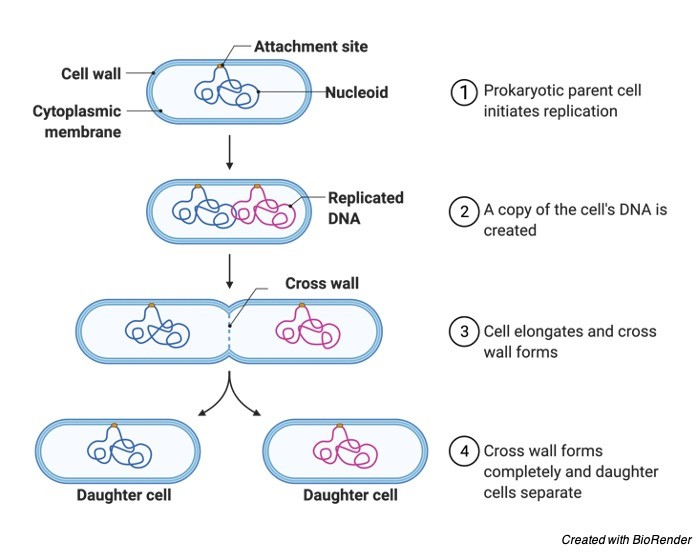
\includegraphics[width=0.7\textwidth]{Fig1.4.png}
\end{figure}

\subsection{Membrane structure}
\begin{und}
    Phospholipids from bilayers in water due to the amphipathic properties of phospholipids molecules. 
\end{und}
\begin{tcolorbox}\begin{que}
    \textbf{Outline the disposition of the phospholipids in the cell membrane.}
    \begin{enumerate}
        \item Water surrounds the cell membrane.
        \item A phospholipid attracted to water with its head/phosphate {\color{red}{$\rightarrow$ hydrophilic}}.
        \item The tails face away the water as they are made of hydrocarbon chains and are apolar. {\color{red}{$\rightarrow$ hydrophobic}}.
        \item A second layer is arranged in an opposite fashion creating a bilayer. 
        \item Phospholipids are \textbf{\color{red}{amphipathic}}.
        \begin{multicols}{2}
        \begin{figure}[H]
            \center
            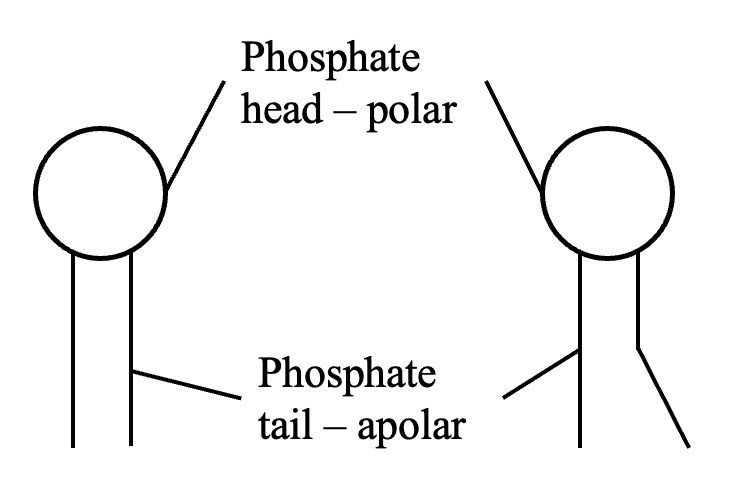
\includegraphics[width=0.35\textwidth]{Fig1.5.png}
        \end{figure}
        \setchemfig{atom sep=2em}
        \chemfig{O^{-}-P([:-90]=O)([:90]=O)-C([:-90]-C([:0]-CH_2-{(}CH_2{)}_n-CH_2))([:90]-C([:0]-CH_2-{(}CH_2{)}_n-CH_2))}
        \end{multicols}
    \end{enumerate}
\end{que}\end{tcolorbox}
\begin{skl}
    Drawing fluid mosaic model. 
    \begin{figure}[H]
        \center
        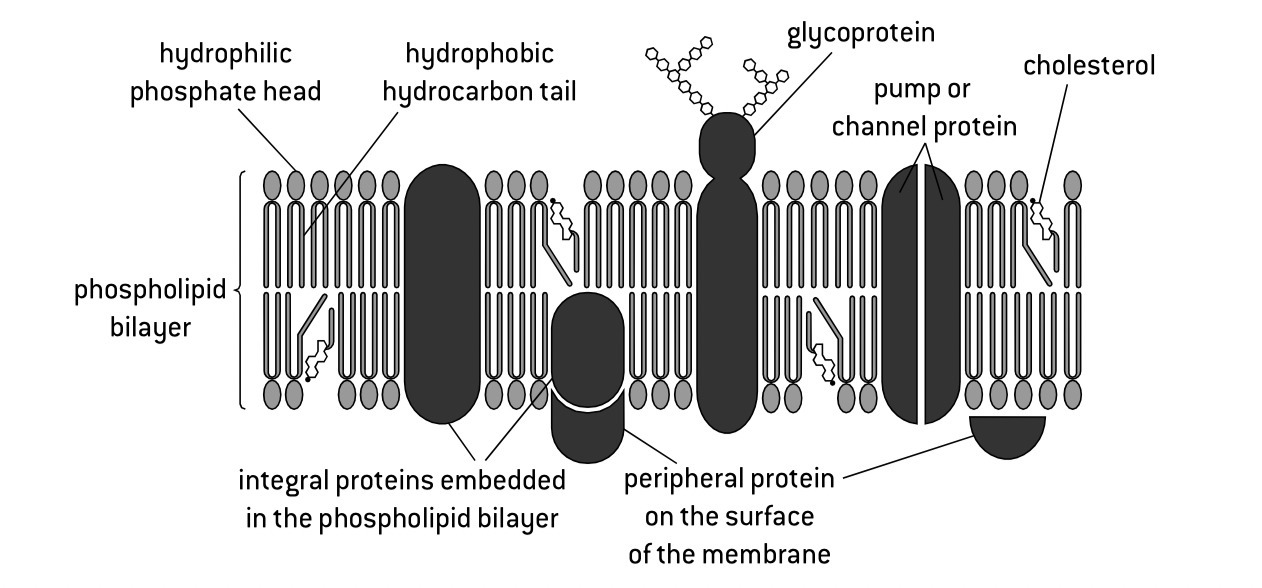
\includegraphics[width=\textwidth]{Fig1.6.png}
    \end{figure}
\end{skl}
\textbf{Movement of phospholipids}
\begin{itemize}
    \item Lateral movement - many times
    \item Flip-flop - barely happen
\end{itemize}
\begin{und}
    Membrane proteins are diverse in terms of structure, position in the membrane, and fucntion. 
\end{und}
\begin{enumerate}
    \item Hormone binding sites
    \item Immobilized enzymes
    \item Cell adhesion
    \item Cell-to-cell communication
    \item Channels for passive transport
    \item Pumps for active transport
\end{enumerate}
\begin{und}
    \textbf{\color{red}{Cholesterol}} is a component of animal cell membranes. 
\end{und}
\begin{enumerate}
    \item \begin{app} Cholesterol in mammalian membranes reduces membrane fluidity and permeability to some solutes. \end{app}
    \item Cholesterol is amphipathic: it has a ---OH group, which is polar. 
\end{enumerate}
\begin{skl}
    Analysis of evidence from electron microscopy that led to the proposal of the Davson-Danielli model.
\end{skl}
\textbf{Evidence: Microscope observation}
\begin{figure}[H]
    \center
    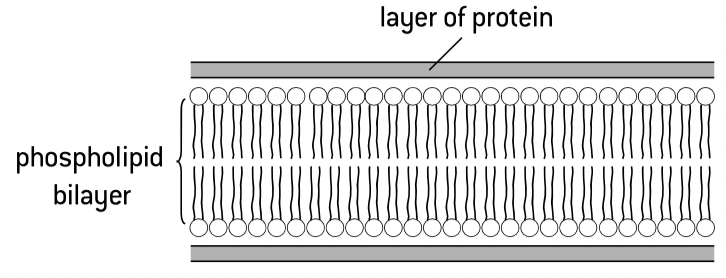
\includegraphics[width=0.7\textwidth]{Fig1.7.png}
\end{figure}
\begin{skl}
    Analysis of the falsification of the Davson-Danielli model that led to the Singer-Nicolson model.
\end{skl}
\begin{enumerate}
    \item Freeze-etched electron micrographs
    \item Structure of membrane proteins
    \item Fluorescent antibody tagging
\end{enumerate}

\subsection{Membrane transport}
\begin{und}
    Particles move across membranes by simple diffusion, facilitated diffusion, osmosis, and active transport. 
\end{und}
\begin{enumerate}
    \item \textbf{\color{red}{Passive transport}}: ATP is not required. {\color{blue}{Diffusion, osmosis, facilitated diffusion.}}\\\textbf{\color{red}{Active transport}}: ATP required. 
    \item \textbf{\color{red}{Simple diffusion}}: Movement of solute particles \textbf{down the concentration gradient}, requires no energy. 
    \item \textbf{\color{red}{Osmosis}}: 
    \begin{itemize}
        \item Df: Passive \textbf{movement of water} across a \textbf{partially/selectively permeable membrane} from a region with \textbf{low solute concentration to a region of high solute concentration}.
        \begin{multicols}{2}
            \begin{figure}[H]
            \center
            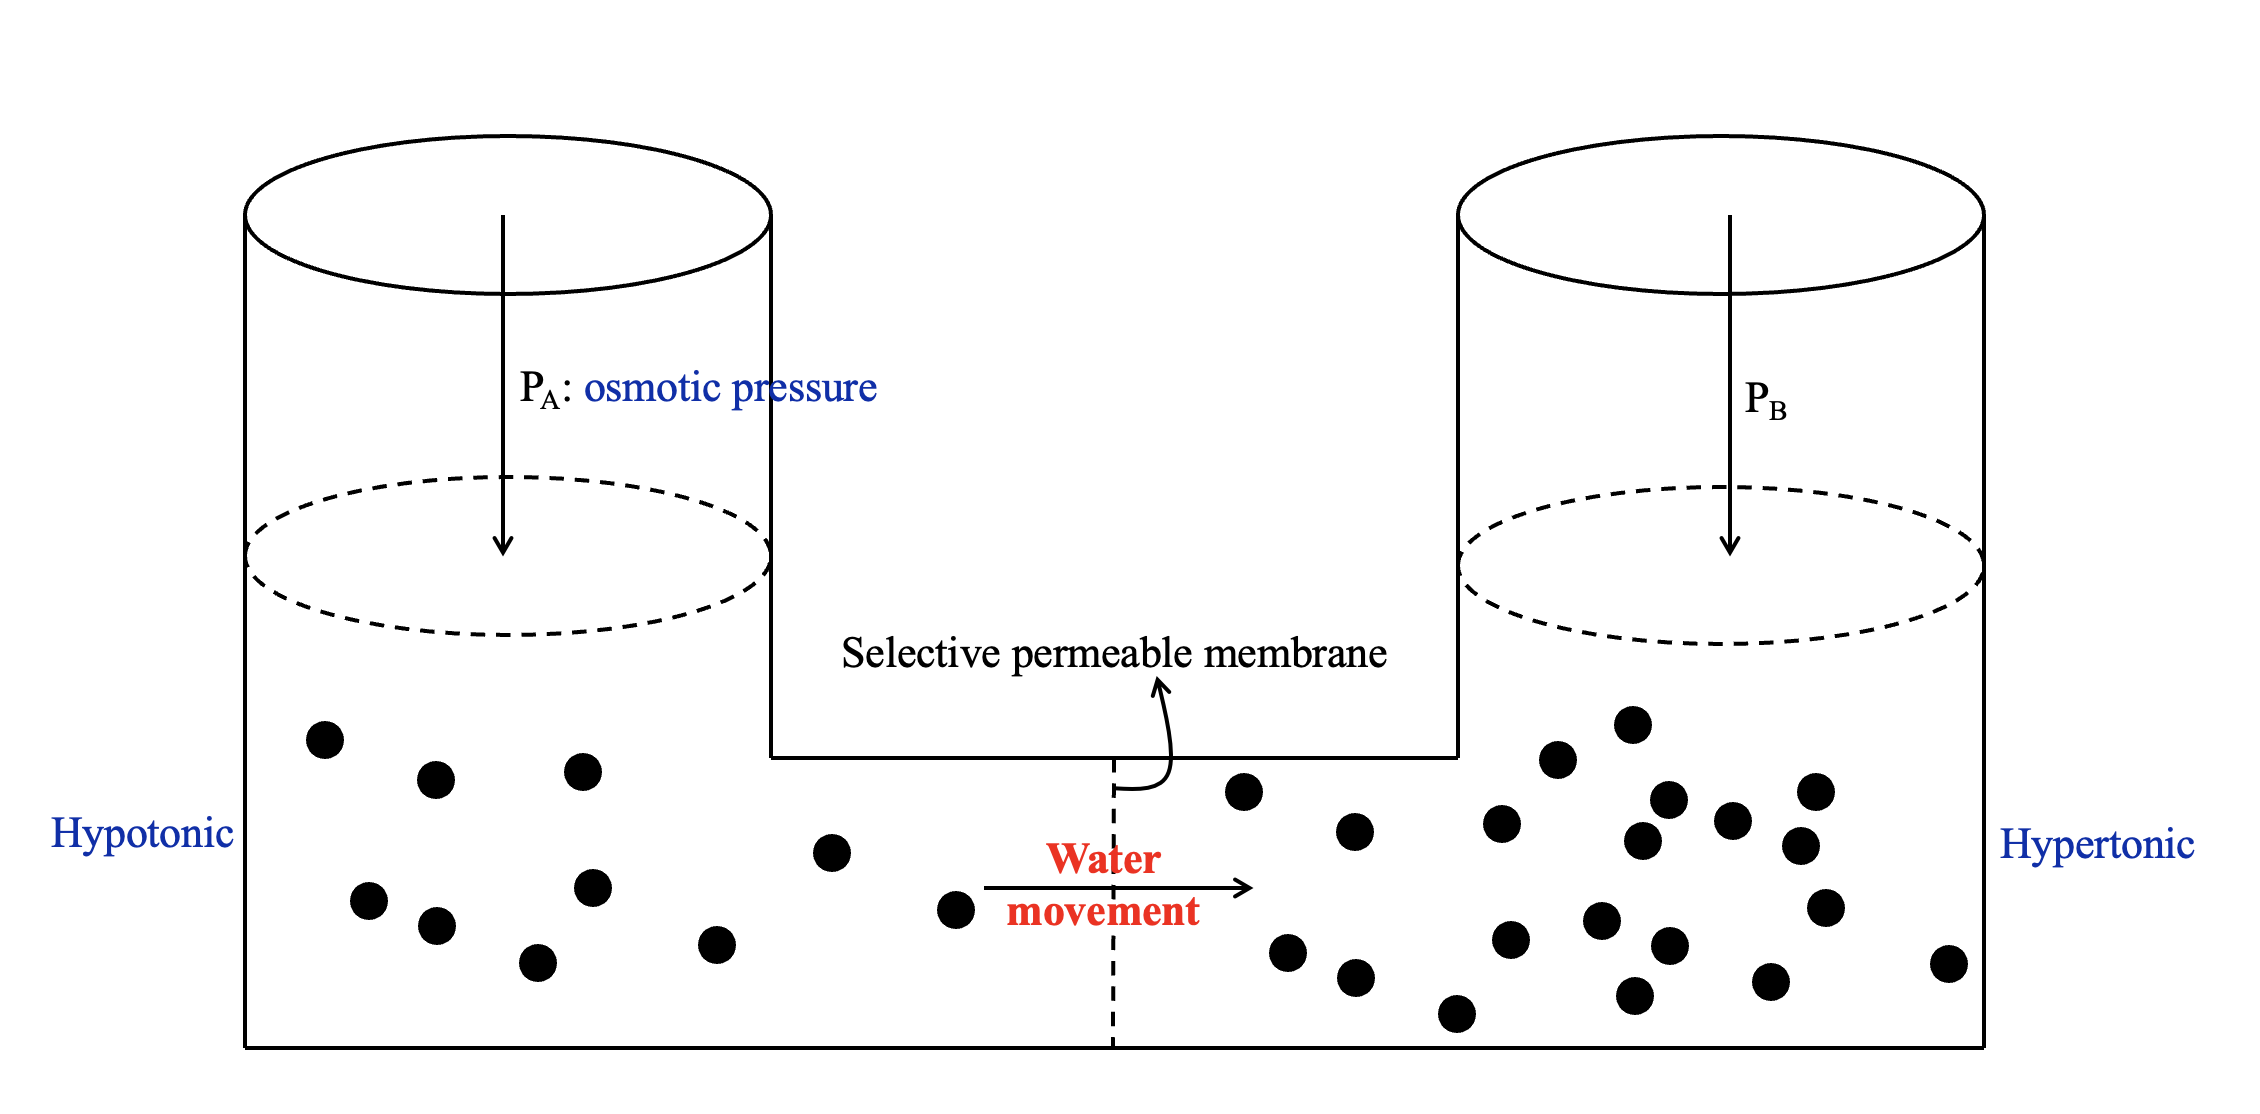
\includegraphics[width=0.45\textwidth]{Fig1.8.png}
        \end{figure}
        \begin{figure}[H]
            \center
            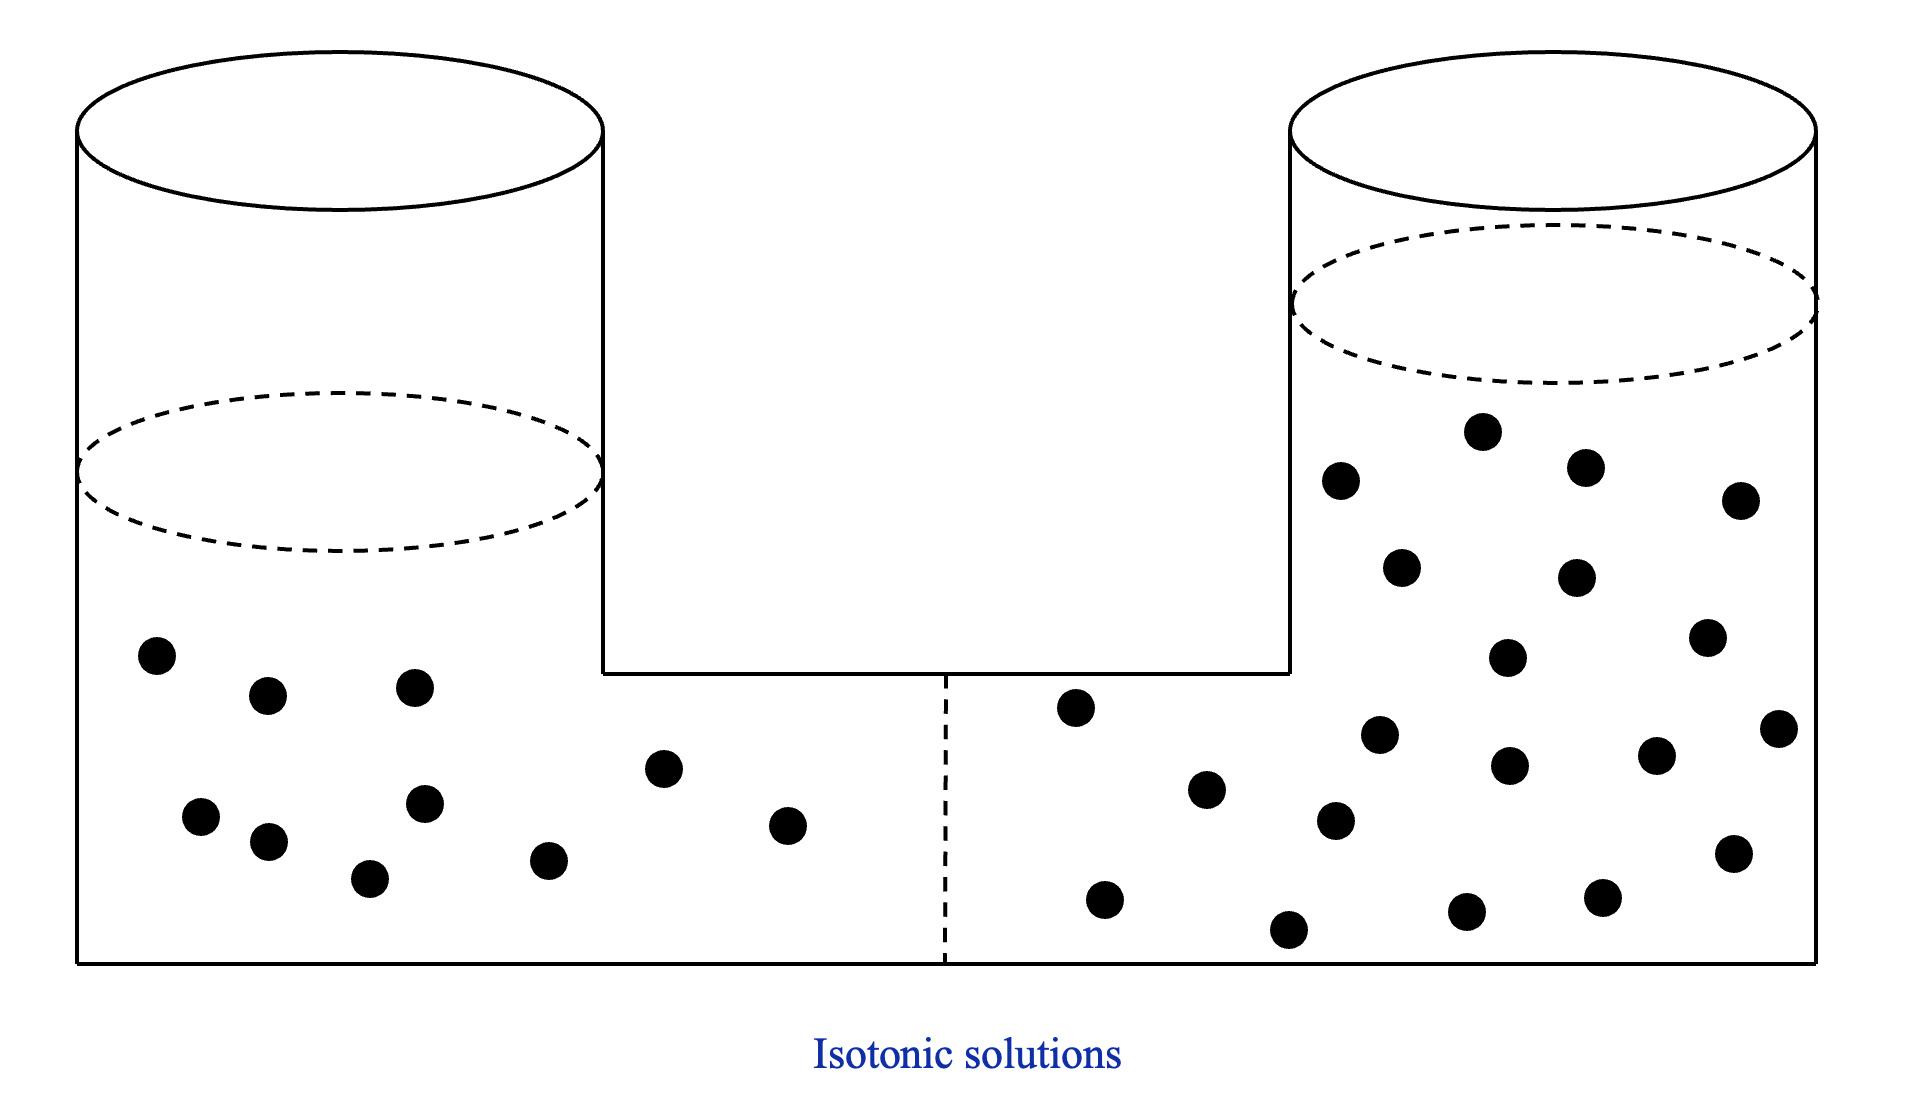
\includegraphics[width=0.41\textwidth]{Fig1.9.png}
        \end{figure}
    \end{multicols}
    \begin{figure}[H]
        \center
        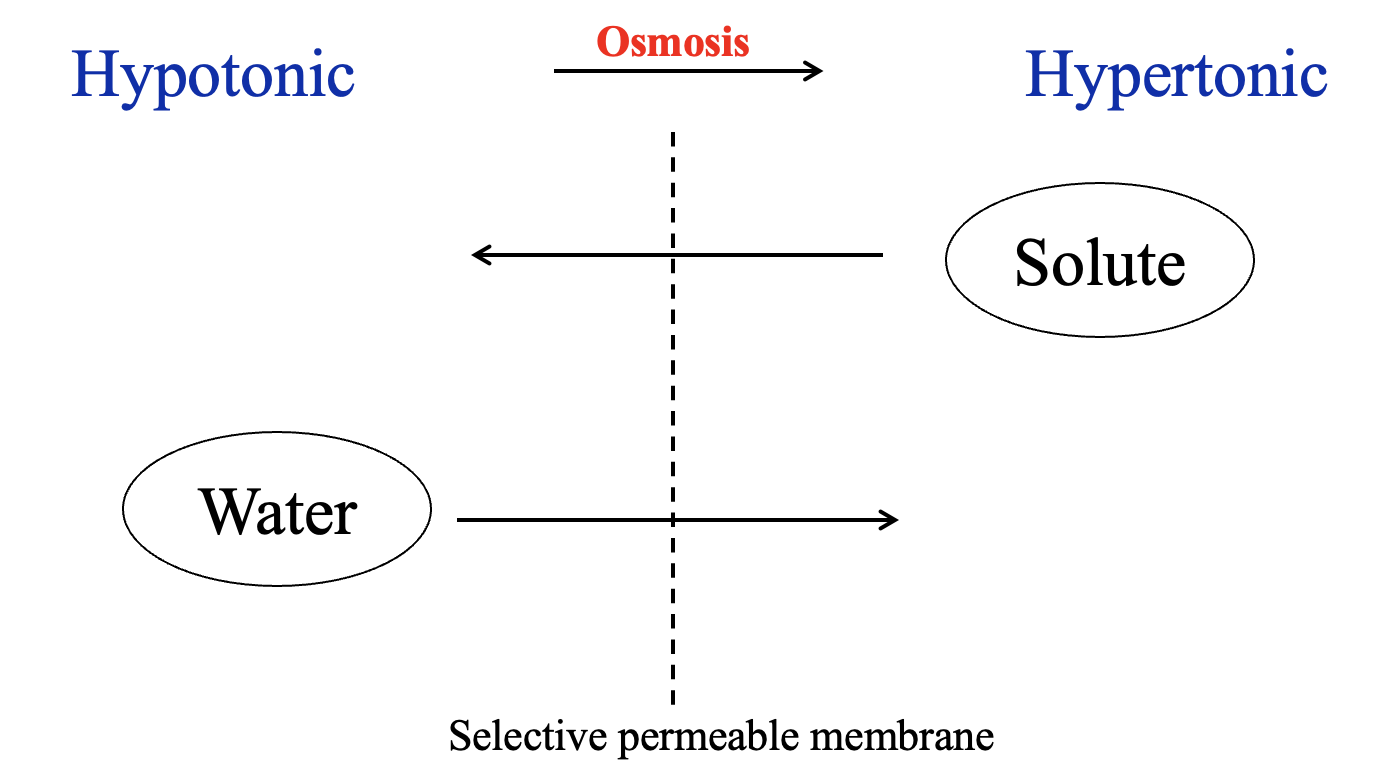
\includegraphics[width=0.5\textwidth]{Fig1.10.png}
    \end{figure}
        \item \textbf{Hypotonic solution}: low water potential inside. \\ \textbf{Isotonic solution}: same water potential. \\ \textbf{Hypertonic solution}: high water potential inside.
        \begin{figure}[H]
            \center
            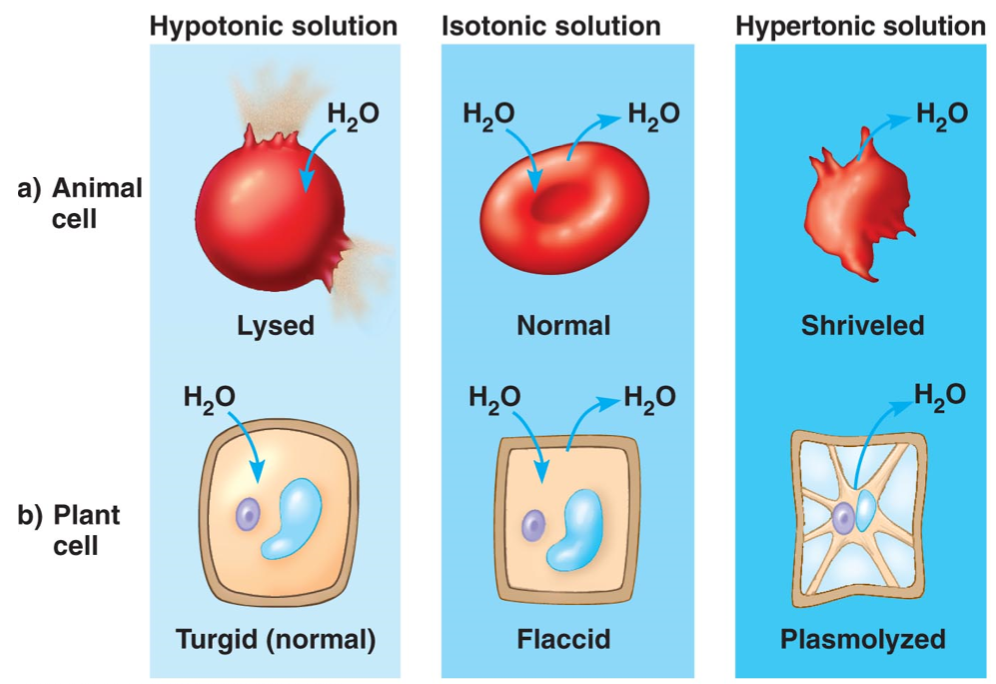
\includegraphics[width=0.5\textwidth]{Fig1.11.png}
        \end{figure}
    \end{itemize}
    \item \textbf{\color{red}{Facilitated transport}}: 
    \begin{itemize}
        \item Df: Movement of solute particles from a concentrated area to a lower one with facilitation of channel proteins, requires no energy. 
        \item The channel only works in one direction; thus, cells need another channel or other ways to excrete them. \\ {\color{blue}{These molecules need a channel protein because they are too big to pass the plasma membrane, or they have a charge.}}
        \begin{figure}[H]
            \center
            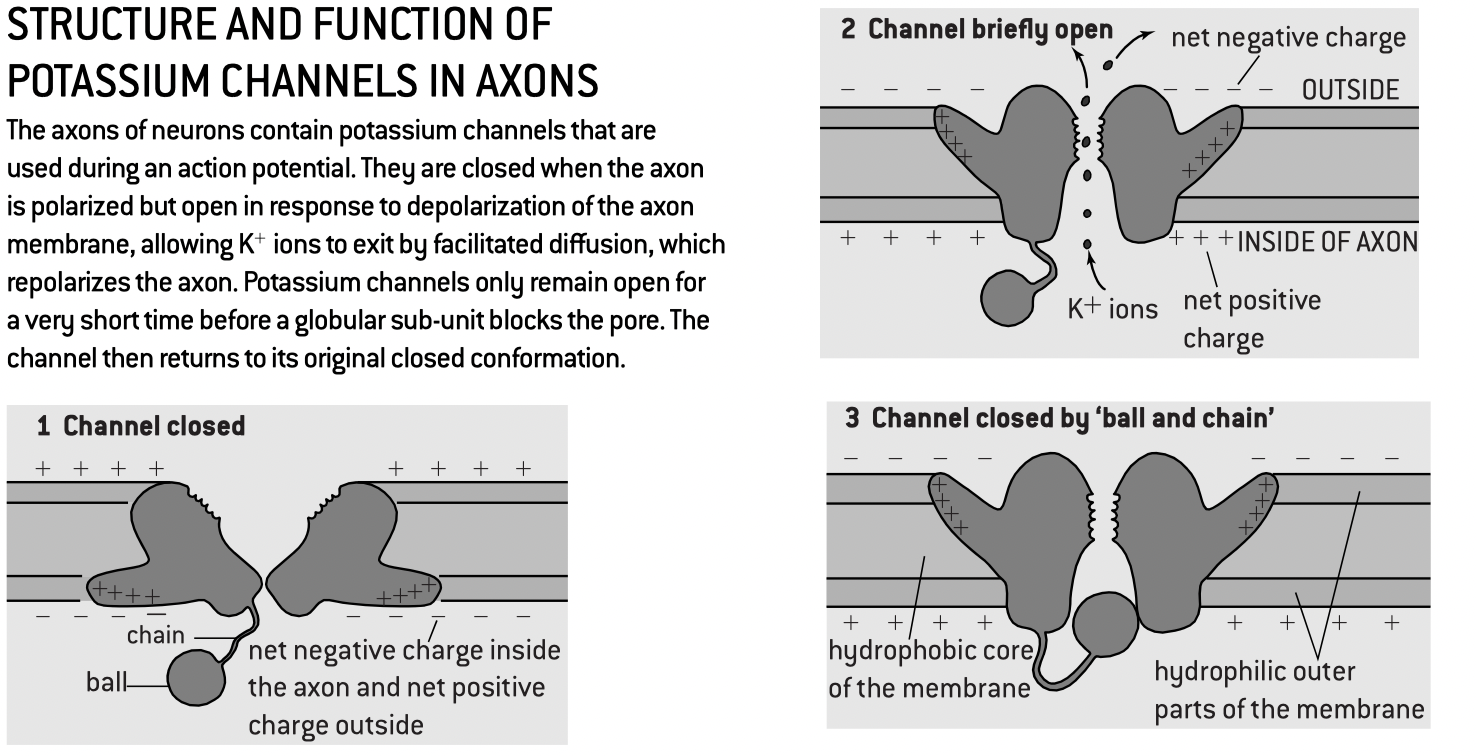
\includegraphics[width=0.75\textwidth]{Fig1.12.png}
        \end{figure}
    \end{itemize}
    \item \textbf{\color{red}{Active transport}}: A movement of solute \textbf{against concentration gradient} with \textbf{expenditure of energy} using a \textbf{protein pump}. 
    \begin{figure}[H]
            \center
            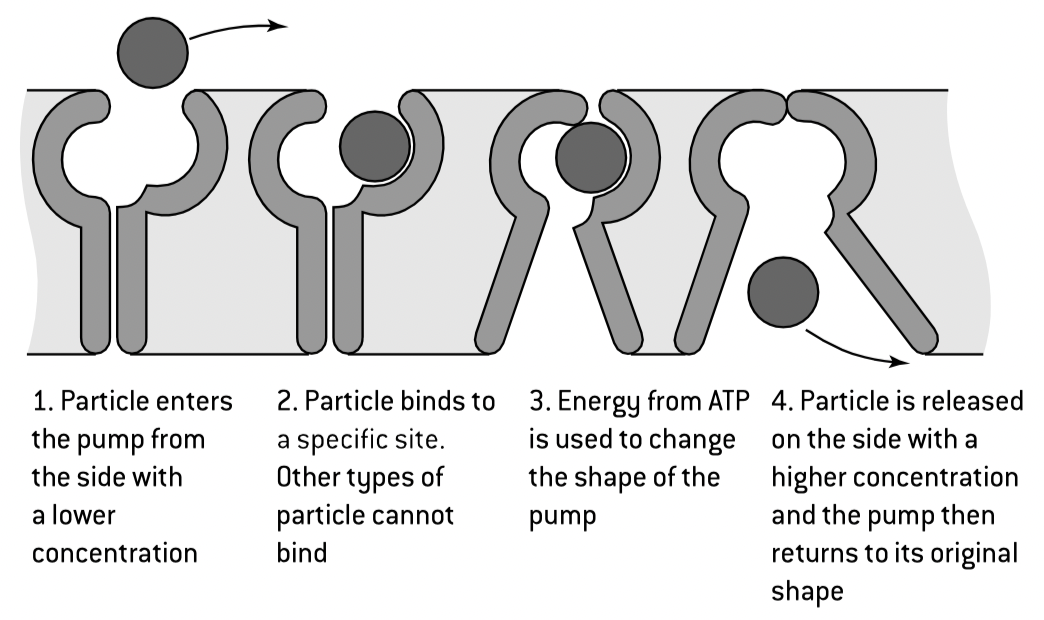
\includegraphics[width=0.75\textwidth]{Fig1.13.png}
    \end{figure}
    {\color{blue}{This transport works against the concentration gradient because the molecules are vital to the cells that they cannot afford to lose one (for example, glucose for animal cells and nitrogen for plant cells.)}}
\end{enumerate}
\begin{app}
    Structure and function of sodium-potassium pumps for active transport and potassium channels for facilitated diffusion in axons. 
\end{app}
\begin{enumerate}
    \item Neurons: 
    \begin{figure}[H]
        \center
        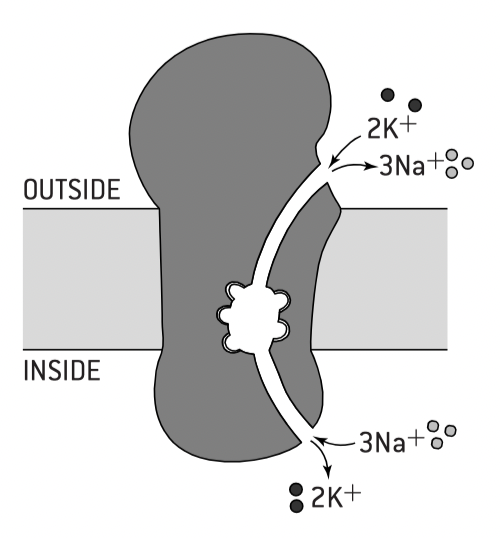
\includegraphics[width=0.4\textwidth]{Fig1.14.png}
    \end{figure}
    \item The Na$^+$ / K$^+$ pump removes 3 Na$^+$ outside the cell and takes 2 K$^+$ in by using one ATP at the same time. 
    \item Purpose: maintain the resting potential for reactions. 
\end{enumerate}
\begin{und}
    The fluidity of membranes allows materials to be taken into cells by endocytosis or exocytosis. Vesicles move materials within cells. 
\end{und}
\begin{enumerate}
    \item \textbf{\color{red}{Exocytosis}}: active transport
    \begin{figure}[H]
        \center
        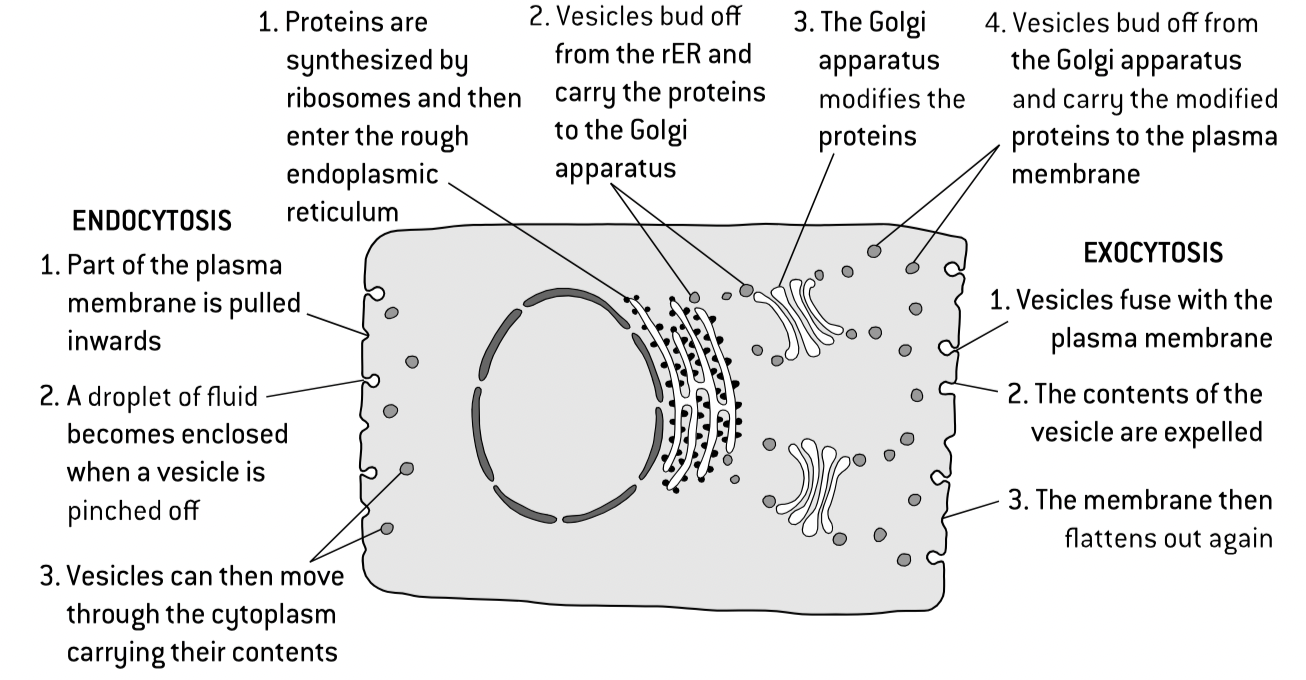
\includegraphics[width=0.9\textwidth]{Fig1.15.png}
    \end{figure}
    \item \textbf{\color{red}{Endocytosis}}: 
    \begin{itemize}
        \item \textbf{Phagocytosis}: cell eating (active transport)\\ A cell projects its cytoplasm to surround a bacterium or a ford particle. Then, it engulfs the particle with its cytoplasm. Once it is inside, the vesicle containing the bacterium will fuse with another vesicel, creating a lysosome. The food item will be digested.
        \item \textbf{Pinocytosis}: cell drinking 
    \end{itemize}
\end{enumerate}
\begin{app}
    issues or organs to be used in medical procedures must be bathed in a solution with the same osmolarity as the cytoplasm to prevent osmosis.
\end{app}
\begin{skl}
    Estimation of osmolarity in tissues by bathing samples in hypotonic and hypertonic solutions. (Practical 2)
\end{skl}
\begin{figure}[H]
    \center
    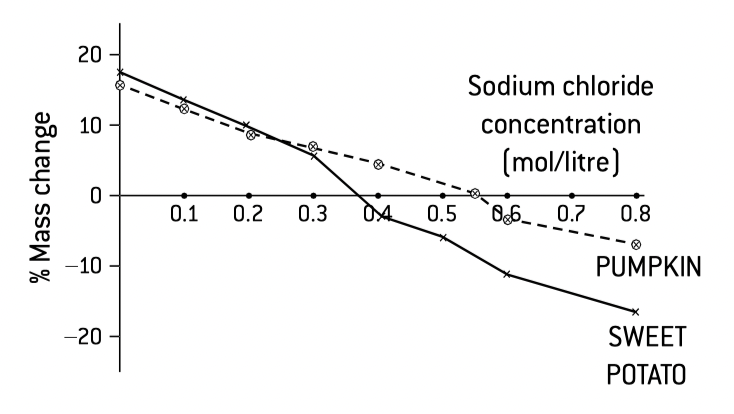
\includegraphics[width=0.55\textwidth]{Fig1.16.png}
\end{figure}

\subsection{The origin of cells}
\begin{und}
    Cell can only be formed by division of pre-existing cells: {\color{blue}{cell division and binary fission. }}
\end{und}
\begin{und}
    The first cells must have arisen from \textbf{non-living} material.
\end{und}
\begin{enumerate}
    \item \begin{app} Miller/Urey Experiment (Pasteur's experiment) \end{app}
    \item Evidence from Pasteur's experiments that spontaneous generation of cells and organisms does not now occur on Earth. 
\end{enumerate}
\begin{und}
    Origin of eukaryotic cells can be explained by the \textbf{endosymbiotic theory}. 
\end{und}
\begin{enumerate}
    \item Compartmentalization: separate different organelles is good for cells.
    \item Endosymbiotic theory: 
    \begin{figure}[H]
        \center
        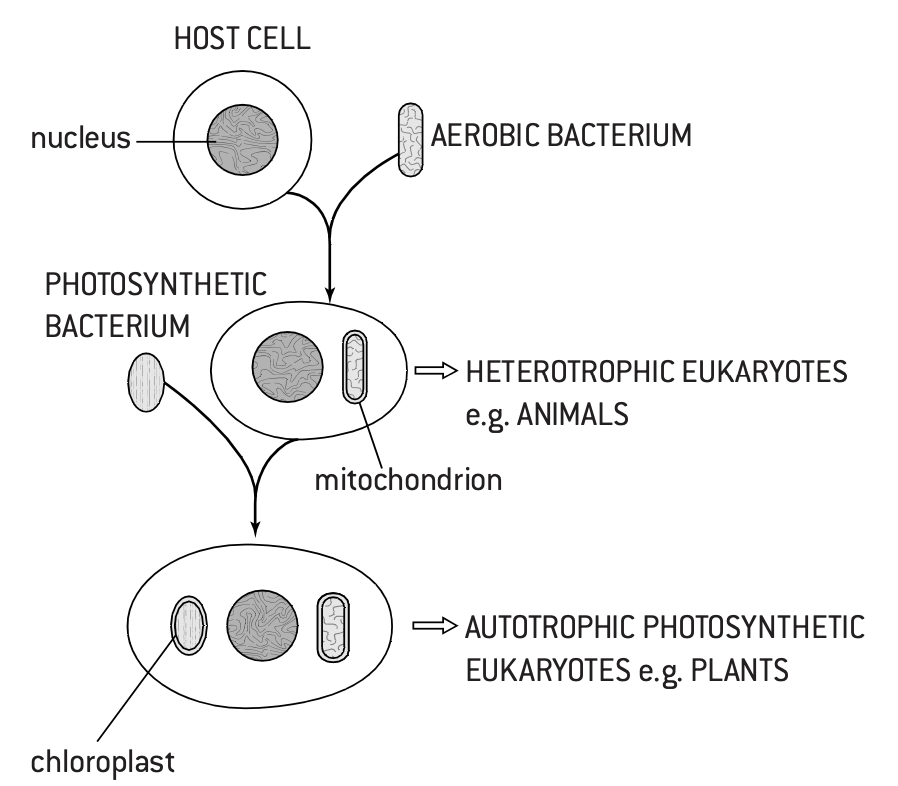
\includegraphics[width=0.55\textwidth]{Fig1.17.png}
    \end{figure}
    \item Evidence: 
    \begin{center}
        \begin{tabular}{c|c|c|c|c}
            \ &Circular DNA&70S ribosomes&Proteins&Binary fission\\
            \hline
            Bacteria&yes&yes&yes&yes\\
            Mitochondria&yes&yes&yes&yes\\
            Chloroplast&yes&yes&yes&yes\\
        \end{tabular}
    \end{center}
\end{enumerate}

\subsection{Cell division}\label{A}
\hyperref[B]{\textbf{Compare this section with \textit{3.3 Meiosis}.}}
\begin{und}
    \textbf{\color{red}{Mitosis}} is division of the nucleus into \textbf{two genetically identical daughter nuclei}. 
\end{und}
\begin{enumerate}
    \item Somatic cell is a cell that has a diploid (2n) number of chromosomes. 
    \item \begin{und} Chromosomes condense by supercoiling during mitosis. \end{und}
    \begin{itemize}
        \item During mitosis S phase, the DNA duplicates. Then, it is arranged as chromosomes. The DNA supercoils, creating condensed bodies called \textbf{chromosomes}.
        \item Draw a homologous pair of chromosomes.
    \end{itemize}
\end{enumerate}

\newpage
\section{Molecular biology}
\subsection{Molecules to metabolism}

\subsection{Water}

\subsection{Carbohydrates and lipids}

\subsection{Proteins}

\subsection{Enzymes}

\subsection{Structure of DNA and RNA}

\subsection{DNA replication, transcription and translation}

\subsection{Cell respiration}

\subsection{Photosynthesis}


\newpage
\section{Genetics}
\subsection{Genes}

\subsection{Chromosomes}

\subsection{Meiosis}\label{B}
\hyperref[A]{\textbf{Compare this section with \textit{1.6 Cell division}.}}


\subsection{Inheritance}

\subsection{Genetic modification and biotechnology}


\newpage
\section{Ecology}
\subsection{Species, communities and ecosystems}
\begin{und}
    \textbf{\color{red}{Species}} are groups of organisms that can potentially interbreed to produce fertile offspring. 
\end{und}
\quad\quad{\color{blue}{e.g. Mules are not considered as a species. }}
\begin{und}
    Members of a species may be reproductively isolated in separate populations
\end{und}
\begin{itemize}
    \item \textbf{\color{red}{Population}}: a group of organisms of the same species living in the same area at the same time. 
\end{itemize}
\begin{und}
    Species have either an autotrophic or heterotrophic method of nutrition. 
\end{und}
\begin{enumerate}
    \item \textbf{\color{red}{Autotroph}}: Organisms which produce their own food from organic molecules. \\ {\color{blue}{e.g.self-feeding, producers}}
    \begin{itemize}
        \item Photoautotroph - {\color{blue}{photosynthesis}}
        \item Chemoautotroph - {\color{blue}{chemosynthesis}}
    \end{itemize}
    \item \textbf{\color{red}{Heterotroph}}: Organisms which derive energy from other living organisms. 
    \begin{itemize}
        \item \textbf{\color{red}{Consumer}}: Ingest organic matter which is living or recently killed. 
        \begin{enumerate}
            \item \textbf{Primary consumer}: eat producers. 
            \item \textbf{Secondary consumer}: eat other consumers/
        \end{enumerate}
        \item \textbf{\color{red}{Decomposer}}: Derive energy from non-living organic matter. 
        \begin{enumerate}
            \item \textbf{\color{red}{Detritivore}}: Ingest non-living organic matter. 
            \item \textbf{\color{red}{Saprotroph}}: Lives in or on non-living organic matter, secreting digestive enzymes into it and absorbing digestive products. 
        \end{enumerate}
    \end{itemize}
\end{enumerate}

\subsection{Energy flow}

\subsection{Carbon cycling}

\subsection{Climate change}


\newpage
\section{Evolution and biodiversity}
\subsection{Evidence for evolution}

\subsection{Natural selection}

\subsection{Classification of biodiversity}

\subsection{Cladistics}


\newpage
\section{Human physiology}
\subsection{Digestion and absorption}

\subsection{The blood system}

\subsection{Defense against infectious disease}

\subsection{Gas exchange}

\subsection{Neurons and synapses}

\subsection{Hormones, homeostasis and reproduction}


\newpage
\section{Nucleic acids}
\subsection{DNA structure and replication}

\subsection{Transcription and gene expression}

\subsection{Translation}


\newpage
\section{Metabolism, cell respiration and photosynthesis}
\subsection{Metabolism}

\subsection{Cell respiration}

\subsection{Photosynthesis}


\newpage
\section{Plant biology}
\subsection{Transport in the xylem of plants}

\subsection{Transport in the phloem of plants}

\subsection{Growth in plants}

\subsection{Reproduction in plants}


\newpage
\section{Genetics and evolution}
\subsection{Meiosis}

\subsection{Inheritance}

\subsection{Gene pools and speciation}


\newpage
\section{Animal physiology}
\subsection{Antibody production and vaccination}

\subsection{Movement}

\subsection{The kidney and osmoregulation}

\subsection{Sexual reproduction}

\end{document}